\begin{lemma} The following holds for roots of unity:
	\begin{enumerate}[label=\thelemma.\arabic*]
		\item $\omega_N^{kN} = 1 \; \forall{k\in \Z}$ \label{lm:roots of unity cyclicity}
		\item $N$ even. $\omega_{N/2} = \omega_N^2$ \label{lm:roots of unity fft}
		\item $\overline{\omega_{N}} = \omega_N^{-1}$ \label{lm:roots of unity conjugate}
		\item $\omega_{N}^{kN/2} = {(-1)}^k \; \forall{k\in \Z}$\label{lm:roots of unity half spin}
	\end{enumerate}
\end{lemma}
\begin{proof} \hfill
	\begin{enumerate}
		\item
		      \[\omega_N^N
			      = {\left(e^{\frac{2\pi i}{N}}\right)}^N
			      = e^{\frac{2\pi iN}{N}}
			      = e^{2\pi i}
			      = \cos(2\pi) + i \sin(2\pi) = 1\]
		      \[\omega_N^{kN}
			      = {\left(\omega_N^{N}\right)}^k = 1^k = 1\]

		\item $\omega_{N/2}
			      = e^{\frac{2\pi i}{N/2}}
			      = e^{2\cdot \frac{2\pi i}{N}}
			      = {\left(e^{\frac{2\pi i}{N}}\right)}^2
			      = \omega_N^2$
		\item $\overline{\omega_{N}}
			      = \overline{e^{\frac{2\pi i}{N}}}
			      = e^{-\frac{2\pi i}{N}}
				      = {\left(e^{\frac{2\pi i}{N}}\right)}^{-1}
			      = \omega_N^{-1}$
		\item $\omega_N^{k\cdot N/2}
			      = {(e^{2\pi i \frac{N/2}{N}})}^k
			      = {(e^{\pi i})}^k = {(-1)}^k$
	\end{enumerate}
\end{proof}

Suppose we have $f: \mathbb{R} \rightarrow \mathbb{C}$ which is $2\pi$-periodic.
Consider the values of this function at points $\frac{0\cdot 2\pi}{N}$,  $\frac{1\cdot 2\pi}{N}$, ..., $\frac{(N-1)\cdot 2\pi}{N}$:
\[x_j:= \frac{j\cdot 2\pi}{N}\]
\[y_j := f(x_j)
	= \sum_{k=-\infty}^\infty \hat{f}(k)e^{ikx_j}
	= \sum_{k=-\infty}^\infty \hat{f}(k)e^{2\pi i\frac{kj}{N}}
	= \sum_{k=-\infty}^\infty \hat{f}(k)\omega_N^{kj}\]

By Lemma~\ref{lm:roots of unity cyclicity} we have that
$\omega_N^{(k+nN)j}
	= \omega_N^{kj}\omega_N^{(nj)N}
	= \omega_N^{kj}$

By grouping the terms with $k_1 = k_2 \mod N$ and obtain the following:

\begin{equation}
	y_j
	= \sum_{k = 0}^{N-1} \omega_N^{kj} \left(\sum_{n=-\infty}^{\infty} \hat{f}(k+nN) \right)
	= \sum_{k =0}^{N-1} \omega_N^{kj} z_k
	\label{eq:IDFT unnormalized}
\end{equation}

We define the matrix $F_{kj} = \frac{1}{\sqrt N} \omega_N^{kj}$. Then:
\begin{equation}
	y_j = \sqrt{N}{(Fz)}_j \Rightarrow
	y = \sqrt{N}Fz \Rightarrow
	z = \frac{1}{\sqrt{N}}F^{-1}y
	= Ty
	\label{eq:DFT unnormalized}
\end{equation}

Later we use the vector $z$ to indicate the output of the DFT, namely $F^{-1}y$

\begin{theorem} \label{thm:DFT unitary}
	The matrix $F_{kj} = \frac{1}{\sqrt N} \omega_N^{kj}$ is unitary
\end{theorem}
\begin{proof}
	\[\begin{aligned}
			{(F \overline{F^T})}_{jl}
			= \frac{1}{\sqrt N}\overline{\left(\frac{1}{\sqrt N}\right)}\sum_{k=0}^{N-1}F_{jk}{(\overline{F^T})}_{kl}
			= \frac{1}{N} \sum_{k=0}^{N-1}F_{jk}\overline{F_{lk}}
			 & = \\ \frac{1}{N} \sum_{k=0}^{N-1}\omega_N^{jk}\overline{\omega_N^{lk}}
			\underset{(a)}{=} \frac{1}{N} \sum_{k=0}^{N-1}\omega_N^{jk}\omega_N^{-lk}
			= \frac{1}{N} \sum_{k=0}^{N-1}\omega_N^{(j-l)k}
		\end{aligned}\]

	In (a) we used the identity $\overline{\omega_N^{lk}} = \omega_N^{-lk}$ from Lemma~\ref{lm:roots of unity conjugate}

	\begin{enumerate}
		\item $j \neq l$. Using the formula for sum of geometric series:
		      \[
			      \sum_{k=0}^{N-1}\omega_N^{(j-l)k}
			      = \frac{1 - {\left(\omega_N^{j-l}\right)}^N}{1 - \omega^{j-l}}
			      = \frac{1 - {\left(\omega_N^{N}\right)}^{j-l}}{1 - \omega^{j-l}}
			      \underset{(a)}{=} \frac{1 - 1^{j-l}}{1 - \omega^{j-l}}
			      = 0\]
		      In (a) we used the identity $\omega_N^{N} = 1$ from Lemma~\ref{lm:roots of unity cyclicity}.
		      The condition $j \neq l$ ensures that the denominator is non-zero, so the expression is well-defined.
		\item $j = l$. Then:
		      \[\sum_{k=0}^{N-1}\omega_N^{(j-l)k}
			      = \sum_{k=0}^{N-1}1
			      = N \Rightarrow
			      {(F \overline{F^T})}_{jl} = \frac{1}{N}N=1\]
	\end{enumerate}

	The matrix $FF^* = I$, so $F$ unitary and $F^{-1}=\overline{F^T}$

	The entries of $F^{-1}$ are given by
	$F^{-1}_{ij} = (\overline{F_{ji}})
		= \frac{1}{\sqrt{N}}\overline{\left(\omega_N^{ji}\right)}
		= \frac{1}{\sqrt{N}}\omega_N^{-ij}$.
\end{proof}

Using the result of Theorem~\ref{thm:DFT unitary} and equations \eqref{eq:DFT unnormalized}, \eqref{eq:IDFT unnormalized} we define the discrete Fourier transform:
\begin{equation}
	z_j
	= {(F^{-1}y)}_j
	= \frac{1}{\sqrt{N}}\sum_{k =0}^{N-1} \omega_N^{-kj} y_k
	\label{eq:DFT} \tag{DFT}
\end{equation}
\begin{equation}
	y_j
	= {(Fz)}_j
	= \frac{1}{\sqrt{N}}\sum_{k =0}^{N-1} \omega_N^{kj} z_k
	\label{eq:IDFT} \tag{IDFT}
\end{equation}

\begin{remark}
	Now we make two remarks about the DFT structure:
	\begin{enumerate}[label = \theremark.\arabic*]
		\item Firstly using DFT of size $n$ we are unable to detect the frequencies above the (n-1)-th one. In fact as the equation \eqref{eq:IDFT unnormalized} suggests, the frequency of the form $k+nN$ with $k\in {0, ..., N-1}$ contributes to the entry with index $k$. However the maximum frequency human ear can process is approximately $20000$, so this issue is handled by choosing an appropriate sample rate, that is usually 44100hz, which is double the maximum frequency which can be detected. The exact reason for it such choice is discussed later. The following plot illustrates the issue discussed (so-called aliasing):
		      \begin{figure}[htbp]
			      \centering
			      \begin{tikzpicture}
				      \draw[very thin,color=gray] (-0.1,-1.1) grid (7,1.1);

				      \draw[->] (-0.2,0) -- (7.2,0) node[right] {$x$};
				      \draw[->] (0,-1.2) -- (0,1.2) node[above] {$y$};

				      \draw[color=red, domain=0:2*pi, samples = 20, smooth] plot (\x, {sin(20 * \x r)}) node[above right] {\scriptsize $\substack{\sin(20x) \\ \text{aliased}}$};

				      \foreach \x in {0,...,19} % exaclty 20 point
				      \fill[color = red] (\x * 2 * pi / 19 ,{sin (\x / 19 * 360)}) circle (0.02cm);
			      \end{tikzpicture}

			      \caption{20 discrete points}

			      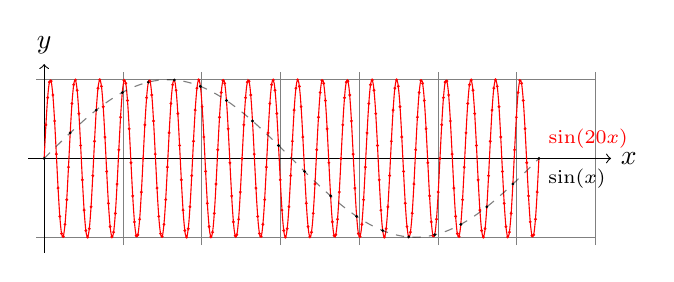
\begin{tikzpicture}
				      \pgfmathsetmacro{\base}{20}
				      \pgfmathsetmacro{\oversample}{15}
				      \pgfmathsetmacro{\count}{(\base-1)*\oversample}

				      \draw[very thin,color=gray] (-0.1,-1.1) grid (7,1.1);

				      \draw[->] (-0.2,0) -- (7.2,0) node[right] {$x$};
				      \draw[->] (0,-1.2) -- (0,1.2) node[above] {$y$};

				      \draw[color=red, domain=0:2*pi + 0.001, samples = \count, smooth] plot (\x, {sin(20 * \x r)}) node[above right] {\scriptsize $\sin(20x)$};

				      \draw[color=black, domain=0:2*pi, samples = \count, smooth, draw opacity=0.5, dashed] plot (\x, {sin(\x r)}) node[below right] {\scriptsize $\sin(x)$};

				      \foreach \x in {0,...,\count}
					      {
						      \pgfmathtruncatemacro{\remainder}{mod(\x, \oversample)}

						      \ifnum\remainder=0  % highlight each point which was present before oversampling
							      \fill[color=black] ({\x * 2 * pi / \count}, {sin(20 * \x / \count * 360)}) circle (0.02cm);
						      \else
							      \fill[color=red] ({\x * 2 * pi / \count}, {sin(20 * \x / \count * 360)}) circle (0.02cm);
						      \fi
					      }
			      \end{tikzpicture}

			      \caption{286 discrete points}
		      \end{figure}
		\item \label{ex:phase shift} The meaning of the phase is often overlooked in the literature, so we consider an example:
		      Let $y = e_k + e_{N-k}$. Then:
		      \[\begin{aligned}
				      Ty
				       & = T_{*k} + T_{*(N-k)}
				      =
				      \begin{pmatrix}
					      \omega_N^{0}  \\
					      \omega_N^{-k} \\
					      \vdots        \\
					      \omega_N^{-k(N-1)}
				      \end{pmatrix}
				      + \begin{pmatrix}
					        \omega_N^{0}      \\
					        \omega_N^{-(N-k)} \\
					        \vdots            \\
					        \omega_N^{-(N-k)(N-1)}
				        \end{pmatrix}
				      \\ &\underset{\text{Lemma \ref{lm:roots of unity cyclicity}}}{=} \begin{pmatrix}
					      \omega_N^{0} + \omega_N^{0}  \\
					      \omega_N^{-k} + \omega_N^{k} \\
					      \vdots                       \\
					      \omega_N^{-k(N-1)} + \omega_N^{k(N-1)}
				      \end{pmatrix}
				      =
				      \begin{pmatrix}
					      2\cos(0)                           \\
					      2\cos\left(\frac{2\pi k}{N}\right) \\
					      \vdots                             \\
					      2\cos\left(\frac{2\pi k(N-1)}{N}\right)
				      \end{pmatrix}
			      \end{aligned}\]
		      As we see from the computation, the output is the function $\cos (kx)$ discretized at points $x_j=\frac{2\pi j}{N}$ for $j\in \{0, \dots, N-1\}$. What happens if we multiply the positive frequency component of $y$ by $\omega_N^{-k}$ and the negative one by $\omega_N^{k}$?
		      \[y^* = \omega_N^{-k}e_k + (\omega_N^{k}e_{N-k})\]
		      \[\begin{aligned}
				      Ty^*
				       & = \begin{pmatrix}
					           \omega_N^{-k} \omega_N^{0} + \omega_N^k \omega_N^{0}  \\
					           \omega_N^{-k} \omega_N^{-k} + \omega_N^k \omega_N^{k} \\
					           \vdots                                                \\
					           \omega_N^{-k} \omega_N^{-k(N-1)} + \omega_N^k \omega_N^{k(N-1)}
				           \end{pmatrix}
				      \\ & = \begin{pmatrix}
					      \omega_N^{-k} + \omega_N^{k}   \\
					      \omega_N^{-2k} + \omega_N^{2k} \\
					      \vdots                         \\
					      \omega_N^{-kN} + \omega_N^{kN}
				      \end{pmatrix} =
				      \begin{pmatrix}
					      2\cos\left(\frac{2\pi k}{N}\right)        \\
					      2\cos\left(\frac{2\pi \cdot 2k}{N}\right) \\
					      2\cos\left(\frac{2\pi \cdot 3k}{N}\right) \\
					      \vdots                                    \\
					      2\cos\left(\frac{2\pi kN}{N}\right)
				      \end{pmatrix}
			      \end{aligned}\]
		      We effectively moved the phase of the cosine by $\frac{2\pi}{N}$, since
		      \[\begin{aligned}
				      {(Ty^*)}_j
				       & = 2\cos\left(\frac{2\pi k(j+1)}{N}\right)
				      = 2\cos\left(k\left(\frac{2\pi j}{N} + \frac{2\pi}{N}\right)\right)
				      \\ &= 2\cos\left(k\left(x_j + \frac{2\pi}{N}\right)\right)
			      \end{aligned}\]

		      not hard yet difficult to see by yourself (at least for me)
	\end{enumerate}
\end{remark}

\begin{theorem}[Real signal conjugate symmetry] \label{thm:real signal symmetry}
	Let $N$ be even. The following are equivalent:

	\begin{enumerate}
		\item $y = \overline{y}, y\in \C^N$
		\item $z_{j} = \overline{z_{N-j}} \quad \forall j \in \{1, \dots, N/2-1\}$ and $z_0, z_{N/2} \in \R$
	\end{enumerate}
\end{theorem}
\begin{proof} \hfill \break
	$"(1)\Rightarrow (2)"$ Using the formula for \ref{eq:DFT}
	\[\begin{aligned}
			z_j
			= \frac{1}{\sqrt N} \sum_{k=0}^{N-1} \omega_N^{-kj}y_k
			= \frac{1}{\sqrt N} \sum_{k=0}^{N-1} \overline{\omega_N^{kj}} y_k
			\underset{y=\overline{y}}{=} \frac{1}{\sqrt N} \sum_{k=0}^{N-1} \overline{\omega_N^{kj}y_k}
			 & = \\ \overline{ \left(\frac{1}{\sqrt N} \sum_{k=0}^{N-1} \omega_N^{kj} y_k \right)}
			\underset{\omega_N^{kN}=1}{=} \overline{ \left(\frac{1}{\sqrt N} \sum_{k=0}^{N-1} \omega_N^{-kN}\omega_N^{kj} y_k \right)}
			 & = \\ \overline{ \left(\frac{1}{\sqrt N} \sum_{k=0}^{N-1} \omega_N^{-k(N-j)} y_k \right)}
			= \overline{z_{N-j}}
		\end{aligned}\]
	\[z_0
		= \frac{1}{\sqrt N} \sum_{k=0}^{N-1} \omega_N^{-k\cdot 0}y_k
		= \frac{1}{\sqrt N} \sum_{k=0}^{N-1} y_k \in \R\]
	By Lemma~\ref{lm:roots of unity half spin}:
	\[z_{N/2}
		= \frac{1}{\sqrt N} \sum_{k=0}^{N-1} \omega_N^{-k N/2}y_k
		= \frac{1}{\sqrt N} \sum_{k=0}^{N-1} {(-1)}^k y_k \in \R\]

	\noindent $"(2)\Rightarrow (1)"$ Using the formula for \ref{eq:IDFT}
	\begin{equation}
		\begin{aligned}
			y_j
			= \frac{1}{\sqrt{N}}\sum_{k =0}^{N-1} \omega_N^{kj} z_k
			= \frac{1}{\sqrt{N}} \left(z_0 + {(-1)}^jz_{N/2} + \sum_{k = 1}^{N/2-1} \omega_N^{kj} z_k + \sum_{l = N/2+1}^{N-1} \omega_N^{lj} z_l\right)
		\end{aligned} \label{eq:real signal symmetry inv 1}
	\end{equation}
	\[\begin{aligned}
			\sum_{k = 1}^{N/2-1} \omega_N^{kj} z_k + \sum_{l = N/2+1}^{N-1} \omega_N^{lj} z_l
			\underset{l'=N-l}{=} \sum_{k = 1}^{N/2-1} \omega_N^{kj} z_k + \sum_{l = 1}^{N/2-1} \omega_N^{(N-l)j} z_{N-l}
			 & = \\ \sum_{k = 1}^{N/2-1} \left(\omega_N^{kj} z_k + \omega_N^{(N-k)j} z_{N-k}\right)
			= \sum_{k = 1}^{N/2-1} \left(\omega_N^{kj} z_k + \overline{\omega_N^{kj}z_k}\right) \in \R
		\end{aligned}\]
	By plugging this expression back to \eqref{eq:real signal symmetry inv 1} we get:
	\[\eqref{eq:real signal symmetry inv 1}
		= \frac{1}{\sqrt{N}} \left(z_0 + {(-1)}^jz_{N/2} + \sum_{k = 1}^{N/2-1} \left(\omega_N^{kj} z_k + \overline{\omega_N^{kj}z_k}\right)\right) \in \R\]
	since all the summands and the factor in front are real.
\end{proof}